\documentclass[a4paper]{article}
\usepackage{amsmath}
\usepackage{graphicx}
\usepackage{longtable}
\usepackage{makecell}
\usepackage[most]{tcolorbox}
\usepackage{listings}
\usepackage{csquotes}

\title{SDCND Advanced Lane Finding}
\date{2019-03-11}
\author{Matthias Schinacher matthias.schinacher@googlemail.com}

\begin{document}

\maketitle
\tableofcontents
\newpage

\section{Intro}
The project is a homework assignment for Udacity's \textbf{Self Driving Car Nano Degree}.
The project is the second one called \textit{Advanced Lane Finding}.

\subsection{Implementation}
I choose to implement the necessary code as a series of python scripts invoked from
the command line, rather than implementing a notebook. I did use however the
example \texttt{example.ipynb} as a starting point for the calibration.
\\
I also used my versions of the solutions to the various quizzes in the course
as a code base for my scripts.
\\
The scripts implement each a specific part of the required task for the
project. Those scripts that produce results used in later stages, use the
standard python \textit{pickle} module to save data as python objects.
\\
The scripts have positional command-line parameters.

\section{Calibration}
I calibrated the \enquote{camera} with the script texttt{calibrate.py}.
It uses the \texttt{cv2} method \texttt{calibrateCamera(...)} to do the actual
calibration and \texttt{findChessboardCorners(...)} to find the image points
required within the given chessboard calibration pictures.
\\
The calibration matrix etc. computed is written to a pickle file and the
scripts allows to save and/or show modified calibration images, onto which
the actual chess board corners (\texttt{findChessboardCorners(...)}).

\paragraph{Script parameters}
:\\
\small
\begin{tabular}{ |c|l|l|c| }
  \hline
Position & Name & Description & Default \\
  \hline
1 & \texttt{show-flag} & show the modified calibration images? & \texttt{False} \\
2 & \texttt{save-flag} & save the modified calibration images? & \texttt{True} \\
3 & \texttt{pickle-file-name} & picke file name & \texttt{calibration.pickle} \\
\hline
\end{tabular}
\normalsize
\textit{(the \enquote{save-flag} is only for the pictures, the pickle file will always be written)}

\paragraph{Graphs}
\textit{(some examples of the chessboard corners found in the calibration images)}
:\\
\begin{tabular}{ |c|c| }
  \hline
  Calibration picture & ... with corners identified \\
  \hline
  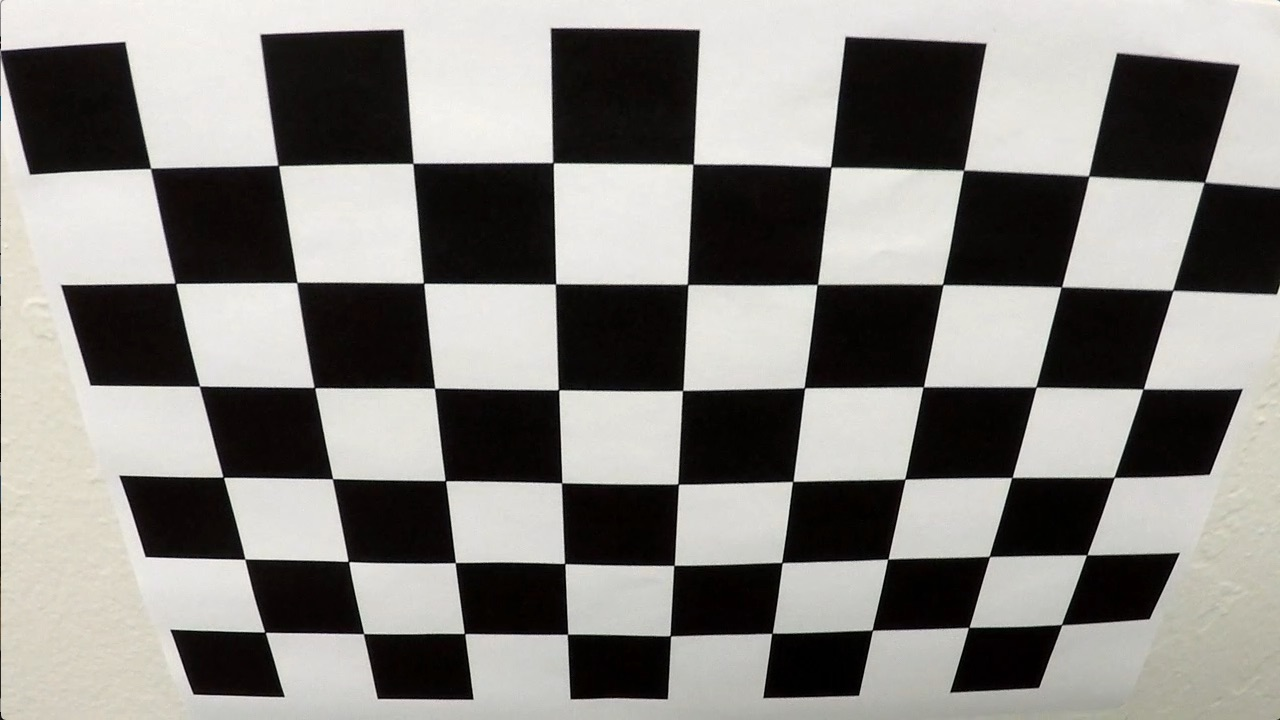
\includegraphics[scale=0.15]{calibration2.jpg} & \includegraphics[scale=0.15]{modcalibration2.jpg} \\
  \hline
  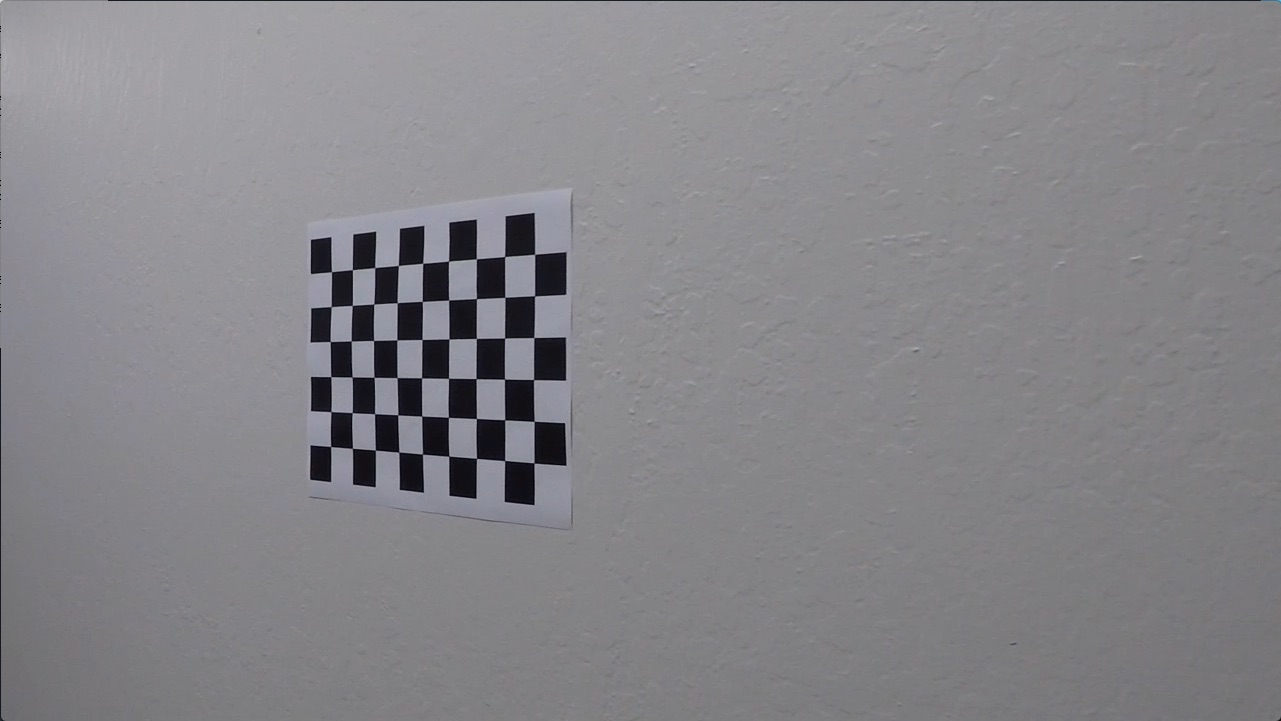
\includegraphics[scale=0.15]{calibration7.jpg} & \includegraphics[scale=0.15]{modcalibration7.jpg} \\
  \hline
  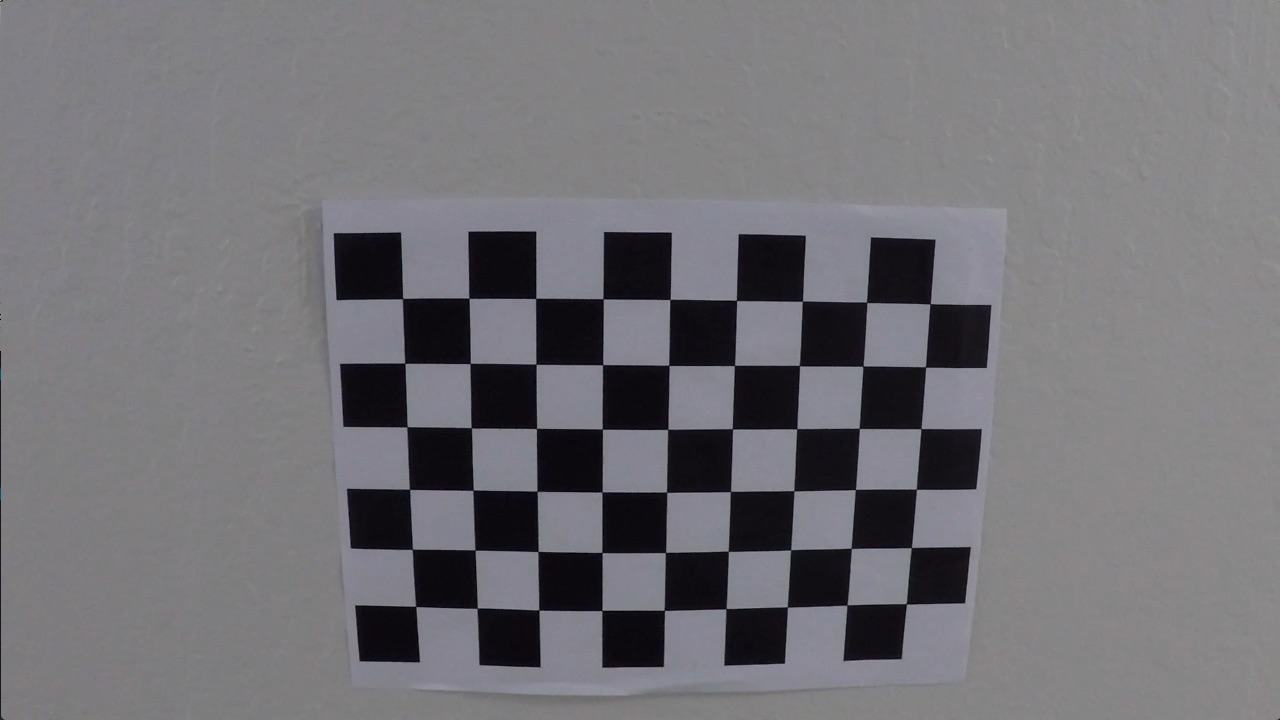
\includegraphics[scale=0.15]{calibration17.jpg} & \includegraphics[scale=0.15]{modcalibration17.jpg} \\
  \hline
\end{tabular}

\textit{(same examples with undistorted images)}
:\\
\begin{tabular}{ |c|c| }
  \hline
  Calibration picture & ... with corners identified \\
  \hline
  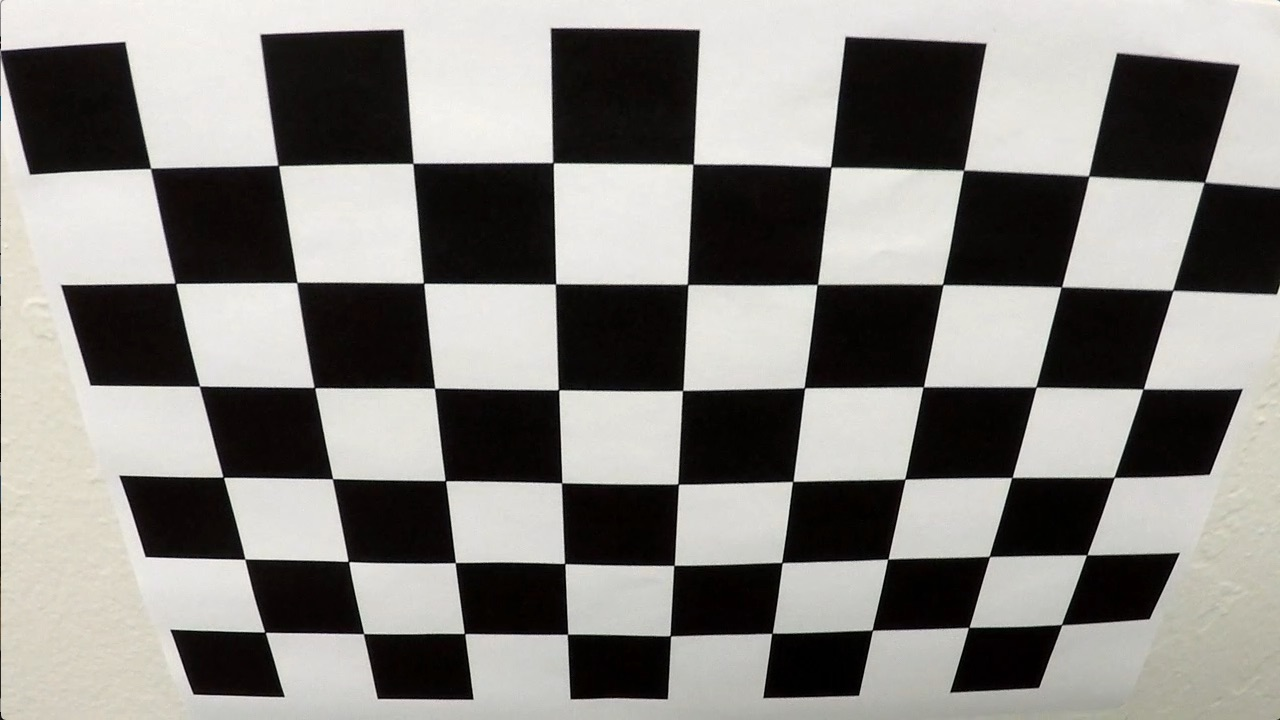
\includegraphics[scale=0.15]{calibration2.jpg} & \includegraphics[scale=0.15]{udcalibration2.jpg} \\
  \hline
  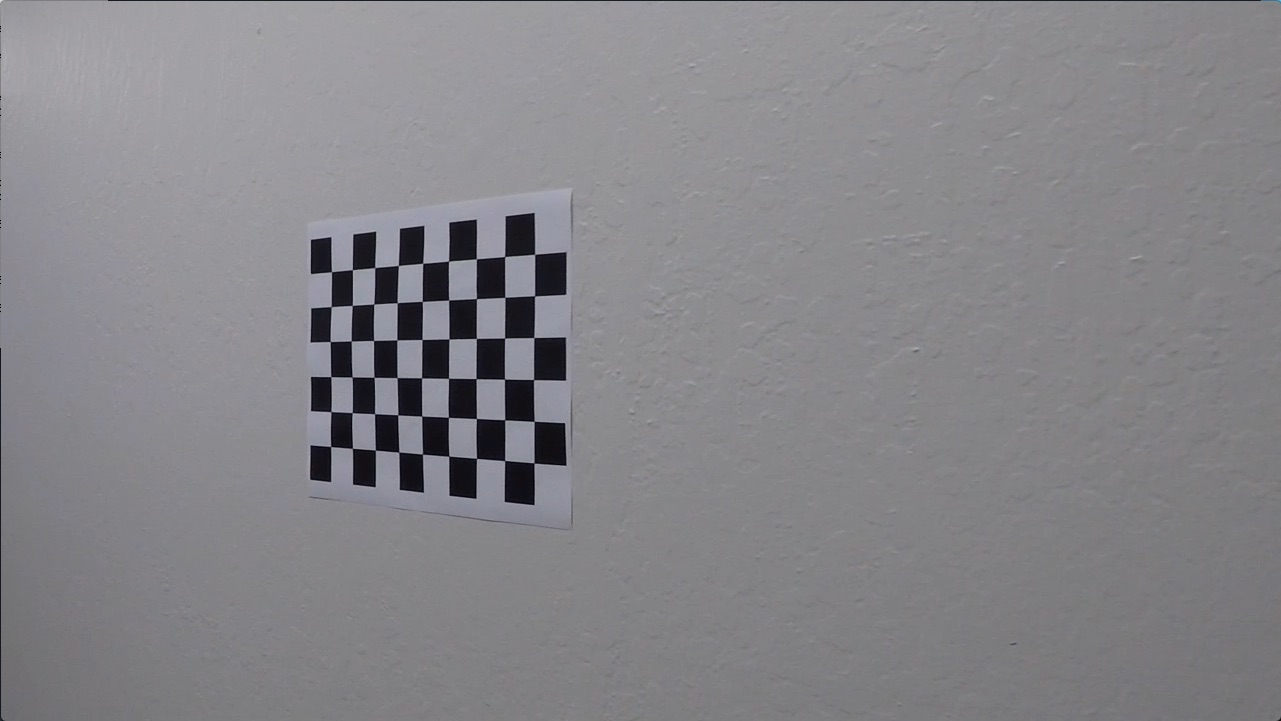
\includegraphics[scale=0.15]{calibration7.jpg} & \includegraphics[scale=0.15]{udcalibration7.jpg} \\
  \hline
  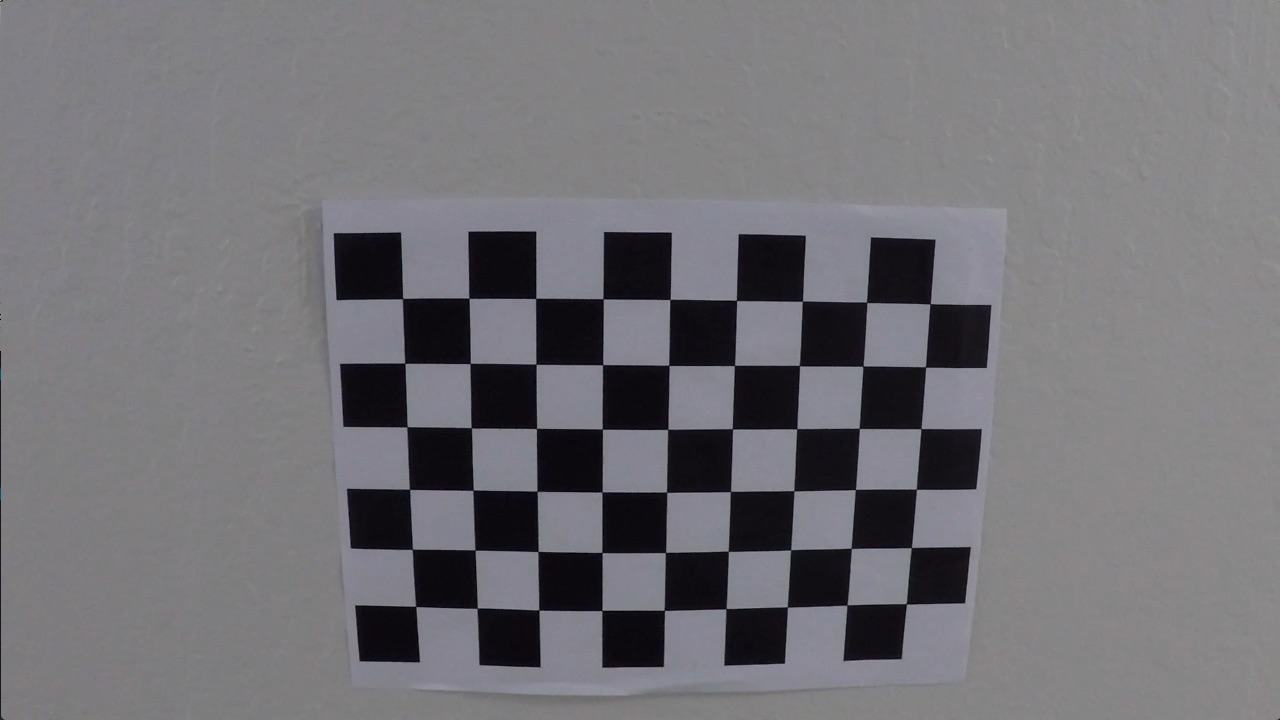
\includegraphics[scale=0.15]{calibration17.jpg} & \includegraphics[scale=0.15]{udcalibration17.jpg} \\
  \hline
\end{tabular}

\section{Perspective transform}
To find a good perspective transform I implemented the script \texttt{transform.py};
It takes as positional input parameters the x and y coordinates for a source quadrilateral
and a destination rectangle defining the desired transform.
\\
Additional parameters control whether to show the test images and how they transform
on the screen and potentially save transformed images and the transformation
parameters (in a pickle file).
\\
This allowed me to experiment with a number of different transformations quite rapidly.
The \enquote{best} transform I came up with \textit{(dubbed \enquote{MA})}, was derived
from the first picture \textit{with straight lines}.
\\
To get the coordinates for the source quadrilateral I would usually open one of
the \textit{straight lines}- pictures with gimp to identify 4 corners that were
not a rectangle but would obviously be close to one in the real. I would then
experiment with a couple of target rectangle coordinates.

\paragraph{Script parameters}
:\\
\small
\begin{tabular}{ |c|l|l|c| }
  \hline
Position & Name & Description & Default \\
  \hline
1 & \texttt{transformation-name} &  & (\textit{mandatory}) \\
2 & \texttt{cooordinate-string} &  & (\textit{mandatory}) \\
3 & \texttt{show-flag} & show images? & \texttt{False} \\
4 & \texttt{save-flag} & save images? & \texttt{False} \\
\hline
\end{tabular}
\normalsize
\\
The coordinates must be given as 16 integers within one string; that requires
the string to be in quotes on the command line, like:\\
\tiny
\texttt{python transform.py MA '425 570 1276 570 806 458 586 458  325 600 1076 600 1076 100 325 100' 1 1}
\normalsize

\paragraph{Graphs}
\textit{(some examples perspective transform; source to transformed picture
with the areas from the transform definition marked.)}
:\\
\begin{tabular}{ |c|c| }
  \hline
  source & transformed \\
  \hline
  \multicolumn{2}{|c|}{\texttt{straight\_lines1.jpg}} \\
  \includegraphics[scale=0.15]{source01.jpg} & \includegraphics[scale=0.15]{transformed01.jpg} \\
  \hline
  \multicolumn{2}{|c|}{\texttt{straight\_lines2.jpg}} \\
  \includegraphics[scale=0.15]{source02.jpg} & \includegraphics[scale=0.15]{transformed02.jpg} \\
  \hline
  \multicolumn{2}{|c|}{\texttt{test3.jpg}} \\
  \includegraphics[scale=0.15]{source03.jpg} & \includegraphics[scale=0.15]{transformed03.jpg} \\
  \hline
\end{tabular}

\section{OTHER}
TODO: Rest of the report

\end{document}
